\documentclass{beamer}

\mode<presentation>
{
\usetheme[width=0.7in]{Hannover}
}
\usepackage{longtable}
\usepackage{booktabs}

\usepackage[english]{babel}
\usepackage[latin1]{inputenc}

\usepackage{times}

\usepackage{multirow}
\usepackage{totpages}
\usepackage{hyperref}
\usepackage{booktabs}

\hypersetup{
  urlcolor=blue,
  linkcolor=blue,
  colorlinks=true
}

\usepackage{listings}
\lstset{columns=flexible,
        language=haskell}
%\usepackage{tikz}
%\usetikzlibrary{positioning}

\usepackage{pgfplots}
\pgfplotsset{width=9cm,height=6cm,compat=1.8}

\newcommand{\blt}{- } %used for bullets in a list

\newcounter{datadefnum} %Datadefinition Number
\newcommand{\ddthedatadefnum}{DD\thedatadefnum}
\newcommand{\ddref}[1]{DD\ref{#1}}

\newcommand{\colAwidth}{0.1\textwidth}
\newcommand{\colBwidth}{0.8\textwidth}

\renewcommand{\arraystretch}{1.1} %so that tables with equations do not look 
%crowded

\pgfdeclareimage[height=0.7cm]{logo}{McMasterLogo}
\title[\pgfuseimage{logo}] % (optional, use only with long paper titles)
{Drasil: A Confluence of Ideas}

\author[]{\underline{Jacques Carette}, Spencer Smith, \ldots}

\institute[McMaster University] % (optional, but mostly needed)
{
  Computing and Software Department\\
  Faculty of Engineering\\
  McMaster University
}

\date[March 12, 2021] % (optional, should be abbreviation of conference name)
{Mila Comp. Calc. RG}

%\subject{computational science and engineering, software engineering, software
%  quality, literate programming, software requirements specification, document
%  driven design}
% This is only inserted into the PDF information catalog. Can be left
% out. 

\pgfdeclareimage[height=0.5cm]{Mac-logo}{McMasterLogo}
\logo{\pgfuseimage{Mac-logo}}

% Delete this, if you do not want the table of contents to pop up at
% the beginning of each subsection:
% \AtBeginSubsection[]
% {
%   \begin{frame}<beamer>
%     \frametitle{Outline}
%     \tableofcontents[currentsection,currentsubsection]
%   \end{frame}
% }

% If you wish to uncover everything in a step-wise fashion, uncomment
% the following command: 

%\beamerdefaultoverlayspecification{<+->}

\beamertemplatenavigationsymbolsempty 

\usepackage{color}

\newcommand{\authornote}[3]{\textcolor{#1}{[#3 ---#2]}}
\newcommand{\jc}[1]{\authornote{purple}{JC}{#1}}

%% Useful abbreviations
\newcommand{\Csharp}{C\#}
\newcommand{\Cplusplus}{C\texttt{++}}

\begin{document}

%%%%%%%%%%%%%%%%%%%%%%%%%%%%%%%%%%%%%%
\hoffset=-.4in %removing side bar for these frames
\begin{frame}[plain]

\titlepage

\end{frame}
\hoffset=0in %restore

%%%%%%%%%%%%%%%%%%%%%%%%%%%%%%%%%%%%%%

\section[Observations]{Observations}

%%%%%%%%%%%%%%%%%%%%%%%%%%%%%%%%%%%%%%

\begin{frame}

\frametitle{Observations}

\begin{enumerate}
  \item<1-> We have good generative technologies
  \item<2-> There are vastly different kinds of software
  \item<3-> ``Software'' is made up of \emph{many} artifacts
  \item<4-> Programmer productivity is a real concern
\end{enumerate}

\end{frame}

%%%%%%%%%%%%%%%%%%%%%%%%%%%%%%%%%%%%%%

\begin{frame}

\frametitle{Generative Technologies}

\textbf{Metaocaml and (typed) template Haskell.}

\begin{itemize}
\item Linear Algebra.
\item Generative Geometry Kernel.
\item Generic Object-Oriented Language.
\item Hakaru.
\item Finally Tagless.
\item Generating Theories ``for free''.
\end{itemize}

\end{frame}

%%%%%%%%%%%%%%%%%%%%%%%%%%%%%%%%%%%%%%

\begin{frame}

\frametitle{Kinds of Software}

\begin{tabular}{|l|l|}
\hline 
\textbf{Kind} & \textbf{Process} \\ \hline\noalign{\pause}
One-off script & Just write it! \\ \hline\noalign{\pause}
Pacemaker software & Design, design, design \\ \hline\noalign{\pause}
Probe O/S (Voyager) & Design, design, design \\ \hline\noalign{\pause}
New project (Uber long ago) & Agile \\ \hline\noalign{\pause}
Linux Kernel & Program Family \\ \hline\noalign{\pause}
\textcolor{blue}{Research Software} & ??? \\ \hline
\end{tabular}

\end{frame}

%%%%%%%%%%%%%%%%%%%%%%%%%%%%%%%%%%%%%%


\begin{frame}

\frametitle{Softifacts}

\begin{itemize}
\item code
\item Makefile (build script / plan)
\item design docs
\item user docs
\item requirements docs
\item tests
\item theory manual
\item installation docs
\end{itemize}
\pause

\textbf{Key Observation}: Different views of the \textcolor{blue}{same}
information
\pause
\textbf{Counterfactual}: If the information wasn't somehow related, why is
it all in the same place?
\pause
\begin{definition}
\emph{Softifacts} are different \textbf{representations} of 
(a subset of) some core knowledge.
\end{definition}

\end{frame}

%%%%%%%%%%%%%%%%%%%%%%%%%%%%%%%%%%%%%%

\begin{frame}

\frametitle{Programmer Productivity}

\end{frame}

%%%%%%%%%%%%%%%%%%%%%%%%%%%%%%%%%%%%%%

\section[Weaving]{Weaving}

%%%%%%%%%%%%%%%%%%%%%%%%%%%%%%%%%%%%%%

\begin{frame}

\frametitle{Requirements}

\begin{itemize}
  \item \textbf{mainstream}: Most potential users
  \uncover<2->{\item \textbf{readable}: Human beings are a target audience}
  \uncover<3->{\item \textbf{idiomatic}: For readability, understandability}
  \uncover<4->{\item \textbf{documented}: For readability, understandability}
  \uncover<5->{\item \textbf{patterns}: More efficient coding}
  \uncover<6->{\item \textbf{expressivity}: Works for real examples}
  \uncover<7->{\item \textbf{common}: Reduce code duplication}
\end{itemize}

\end{frame}

%%%%%%%%%%%%%%%%%%%%%%%%%%%%%%%%%%%%%%

\section[Drasil]{Drasil}

%%%%%%%%%%%%%%%%%%%%%%%%%%%%%%%%%%%%%%

\begin{frame}

\frametitle{Approach}

Start from real OO programs\\~\

\pause

\textcolor{red}{What we can say}
vs. 
\textcolor{blue}{\textbf{want to say}}
vs. 
\textcolor{orange}{need to say}

% \begin{itemize}
% \item Introspection vs. templates vs. function definition
% \end{itemize}

\end{frame}

%%%%%%%%%%%%%%%%%%%%%%%%%%%%%%%%%%%%%%

\begin{frame}[fragile]

\frametitle{Readability Features}

Example: Blocks
\begin{itemize}
  \item Semantically meaningless
  \item Reflect how people write programs
\end{itemize}

\noindent\rule{\textwidth}{1pt}

\begin{lstlisting}[language=Python,basicstyle=\footnotesize]
# Initialize dimensions
h = input('What is the height? ')
w = input('What is the width? ')
d = input('What is the depth? ')

# Calculate volume and surface area
v = h * w * d
sa = 2 * (h * w + w * d + h * d)
\end{lstlisting}
\end{frame}

%%%%%%%%%%%%%%%%%%%%%%%%%%%%%%%%%%%%%%

\begin{frame}

\frametitle{Some ingredients}

\begin{itemize}
  \item Variables distinct from values (viz use/mention)
  \item Smart constructors for common idioms
\end{itemize}

\end{frame}

\end{document}

\section[Implementation]{Implementation}

%%%%%%%%%%%%%%%%%%%%%%%%%%%%%%%%%%%%%%

\begin{frame}[fragile]

\frametitle{Encoding}

Tagless with type families -- 2 Layers of abstraction
\begin{enumerate}
  \item Over target language
  \item Over language-specific representational data structures
\end{enumerate}

\begin{lstlisting}
class (TypeSym repr) => VariableSym repr where
  type Variable repr
  var :: Label -> repr (Type repr)
    -> repr (Variable repr)
\end{lstlisting}

\end{frame}

%%%%%%%%%%%%%%%%%%%%%%%%%%%%%%%%%%%%%%

\begin{frame}
\centering
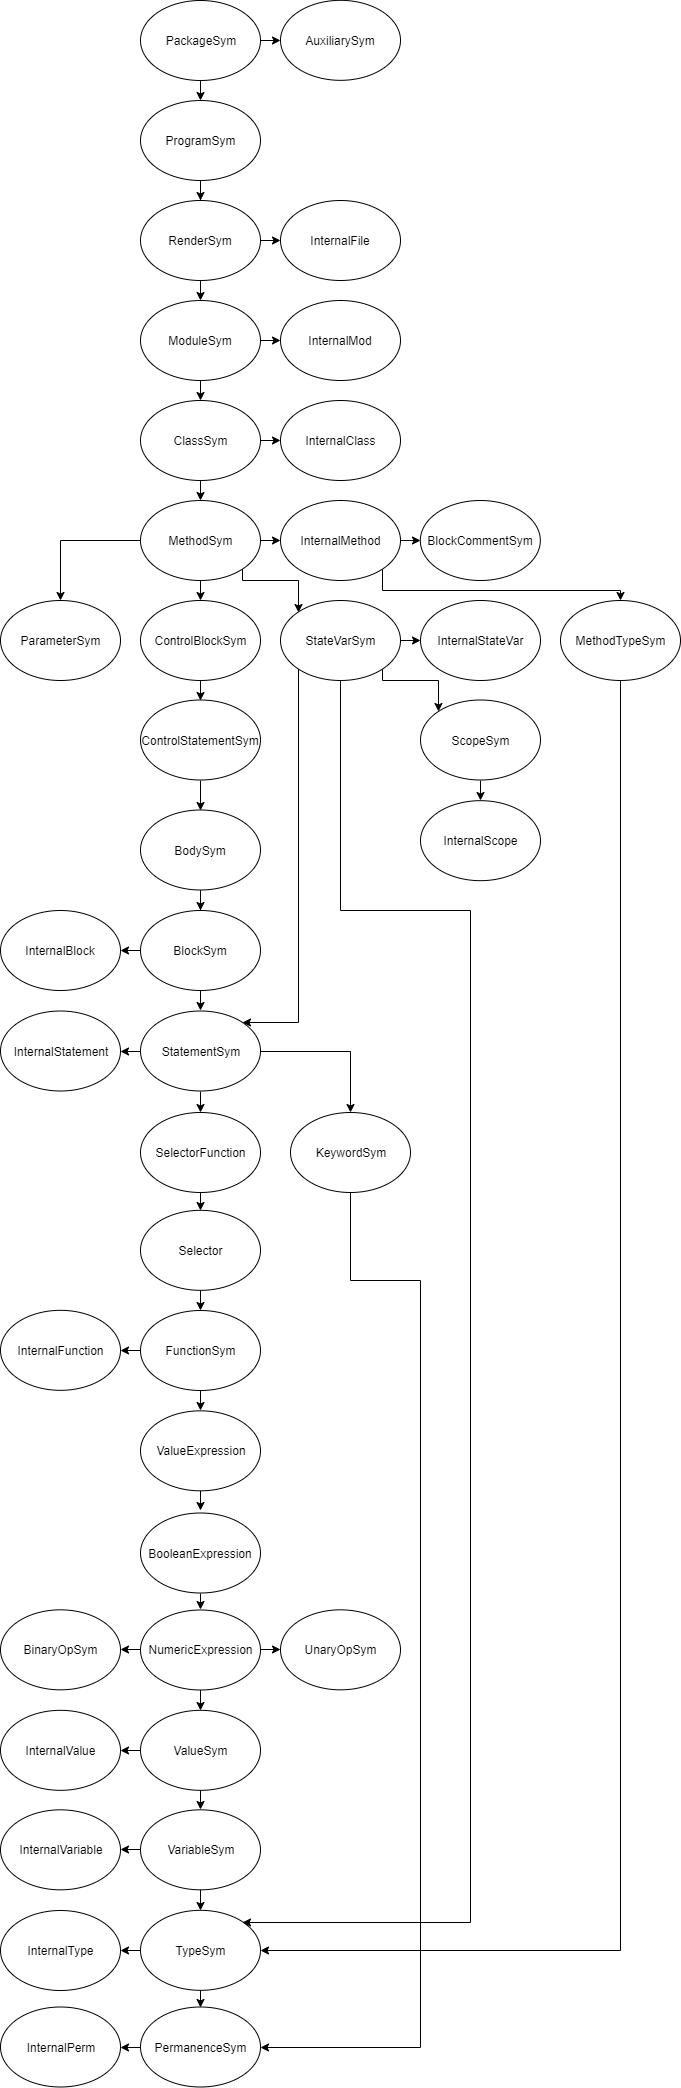
\includegraphics[scale=0.12]{GOOLClasses.png}
\end{frame}

\begin{frame}
\begin{columns}
\begin{column}{0.5\textwidth}
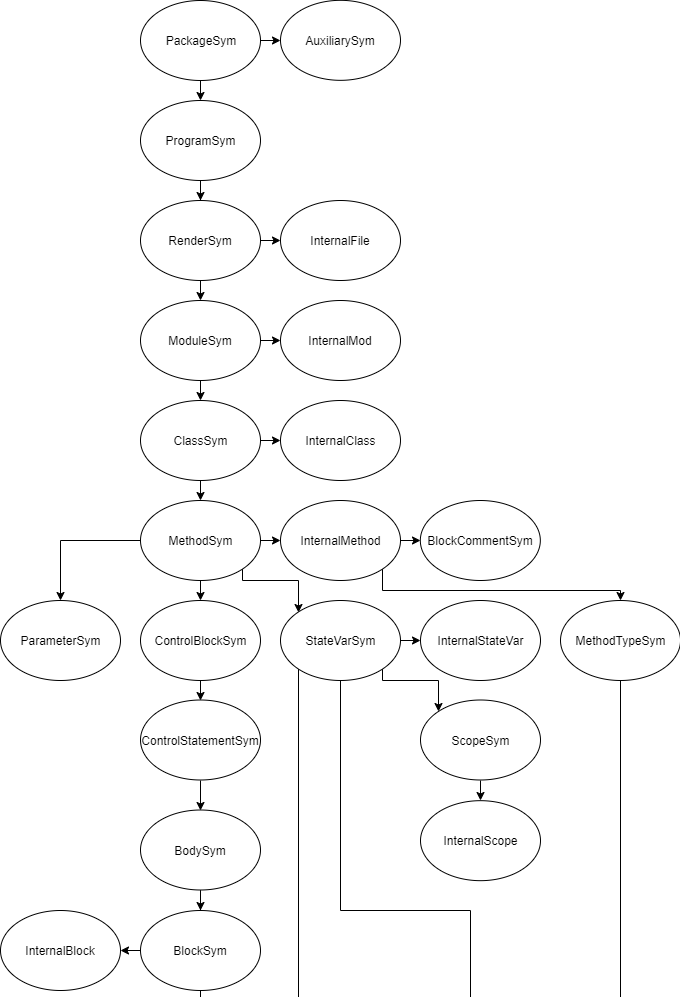
\includegraphics[scale=0.28]{GOOLClasses_top.png}
\end{column}
\begin{column}{0.5\textwidth}
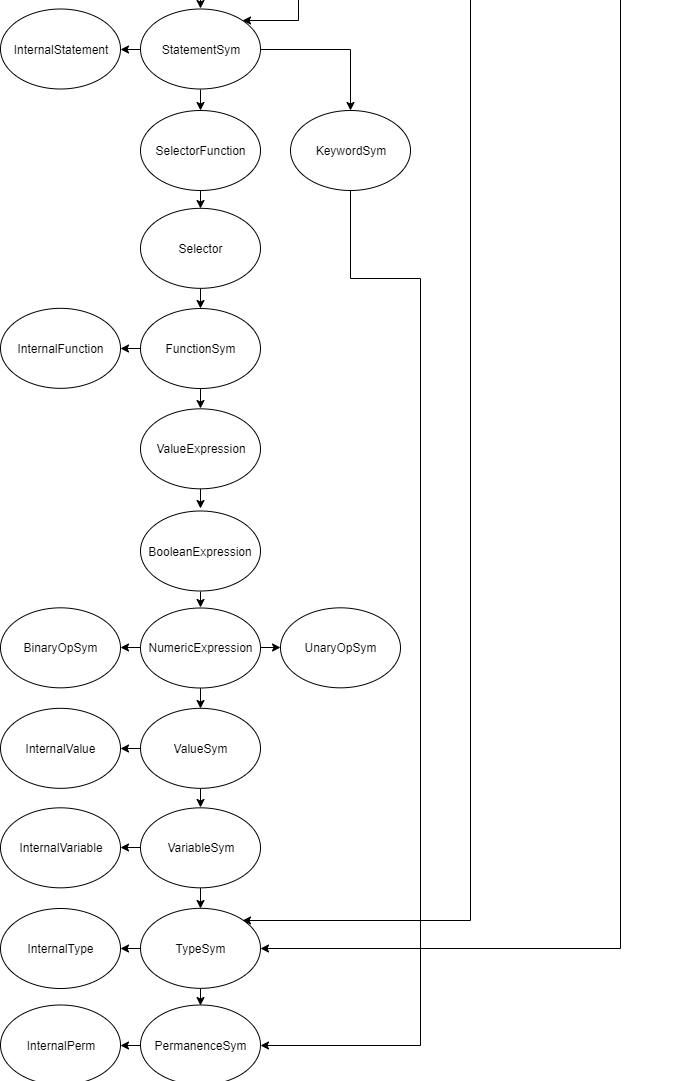
\includegraphics[scale=0.28]{GOOLClasses_bottom.png}
\end{column}
\end{columns}
\end{frame}

%%%%%%%%%%%%%%%%%%%%%%%%%%%%%%%%%%%%%%

\begin{frame}

\frametitle{Statistics}

\begin{itemize}
  \item 43 classes, 328 methods
  \item 300 functions that abstract over commonalities
  \item 40\% more common methods between Java and \Csharp~than Java and Python
\end{itemize}

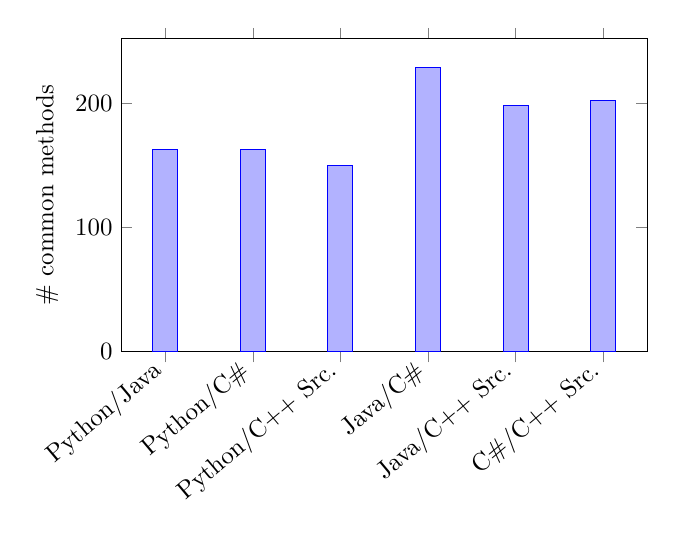
\begin{tikzpicture}[scale=0.9]
\begin{axis}[
ybar,
ymin=0,
ylabel={\# common methods},
symbolic x coords={Python/Java,Python/C\#,Python/C++ Src.,Java/C\#,Java/C++ 
  Src.,C\#/C++ Src.},
xtick=data,
x tick label style={rotate=40,anchor=east},
]
\addplot coordinates {(Python/Java,163) (Python/C\#,163) (Python/C++ Src.,150) 
  (Java/C\#,229) 
  (Java/C++ Src., 198) (C\#/C++ Src., 202)};
\end{axis}
\end{tikzpicture}

\end{frame}

%%%%%%%%%%%%%%%%%%%%%%%%%%%%%%%%%%%%%%

\section[Patterns]{Patterns}

%%%%%%%%%%%%%%%%%%%%%%%%%%%%%%%%%%%%%%

\begin{frame}

\frametitle{Things we need/want to say}

\begin{itemize}
  \item Command line arguments
  \item Lists
  \item I/O
  \item Procedures with Input/Output/Both parameters
  \item Getters and setters
  \item Design patterns
\end{itemize}

\end{frame}

%%%%%%%%%%%%%%%%%%%%%%%%%%%%%%%%%%%%%%

\begin{frame}[fragile]

\frametitle{Example: List Slicing}

GOOL: {\footnotesize \emph{hideous, we know}}
% new list, old list, start value, end value, step size
\begin{lstlisting}
listSlice sliced (valueOf old) (Just $ litInt 1)
  (Just $ litInt 3) Nothing
\end{lstlisting}
\vspace{\baselineskip}

\begin{overprint}
\onslide<1>
Python:
\begin{lstlisting}[language=Python]
sliced = old[1:3:]
\end{lstlisting}

\onslide<2>
Java:
\begin{lstlisting}[language=java]
ArrayList<Double> temp = new ArrayList<Double>(0);
for (int i_temp = 1; i_temp < 3; i_temp++) {
    temp.add(old.get(i_temp));
}
sliced = temp;
\end{lstlisting}

\onslide<3>
\Csharp:
\lstset{language=[Sharp]C}
\begin{lstlisting}
List<double> temp = new List<double>(0);
for (int i_temp = 1; i_temp < 3; i_temp++) {
    temp.Add(old[i_temp]);
}
sliced = temp;
\end{lstlisting}

\onslide<4>
\Cplusplus:
\lstset{language=C++}
\begin{lstlisting}
vector<double> temp(0);
for (int i_temp = 1; i_temp < 3; i_temp++) {
    temp.push_back(old.at(i_temp));
}
sliced = temp;
\end{lstlisting}
\end{overprint}

\end{frame}

\lstset{language=haskell}
%%%%%%%%%%%%%%%%%%%%%%%%%%%%%%%%%%%%%%

\begin{frame}[fragile]

\frametitle{Example: Setters}

GOOL:
\begin{lstlisting}
setMethod "FooClass" foo
\end{lstlisting}
\vspace{\baselineskip}

\begin{overprint}
\onslide<1>
Python:
\begin{lstlisting}[language=Python]
def setFoo(self, foo):
    self.foo = foo
\end{lstlisting}

\onslide<2>
Java:
\begin{lstlisting}[language=java]
public void setFoo(int foo) throws Exception {
    this.foo = foo;
}
\end{lstlisting}

\onslide<3>
\Csharp:
\lstset{language=[Sharp]C}
\begin{lstlisting}
public void setFoo(int foo) {
    this.foo = foo;
}
\end{lstlisting}
\lstset{language=haskell}

\onslide<4>
\Cplusplus:
\begin{lstlisting}[language=C++]
void FooClass::setFoo(int foo) {
    this->foo = foo;
}
\end{lstlisting}
\end{overprint}

\end{frame}

%%%%%%%%%%%%%%%%%%%%%%%%%%%%%%%%%%%%%%

\section[Example]{Example}

%%%%%%%%%%%%%%%%%%%%%%%%%%%%%%%%%%%%%%


\begin{frame}

\frametitle{Complete Example}

As part of
\href{https://jacquescarette.github.io/Drasil/}{Drasil}, we can look at the
Projectile program\\~\

\href{https://github.com/JacquesCarette/Drasil/tree/projectileDemos/Presentations/PEPM2020/projectile1}{Design
 1}
\begin{itemize}
  \item Documented
  \item Bundled inputs
\end{itemize}

\href{https://github.com/JacquesCarette/Drasil/tree/projectileDemos/Presentations/PEPM2020/projectile2}{Design
 2}
\begin{itemize}
  \item Logging
  \item More modular
\end{itemize}

\end{frame}

%%%%%%%%%%%%%%%%%%%%%%%%%%%%%%%%%%%%%%

\section[Current Work]{Current Work}

%%%%%%%%%%%%%%%%%%%%%%%%%%%%%%%%%%%%%%


\begin{frame}

\frametitle{Currently working on}

\begin{itemize}
  \item More types
  \item Smarter generation - ex. import statements
  \item Interfacing with external libraries
  \item User-decisions - ex. which type to use for lists?
  \item More patterns
\end{itemize}

\end{frame}

%%%%%%%%%%%%%%%%%%%%%%%%%%%%%%%%%%%%%%

\begin{frame}

\frametitle{Language of Design}

Drasil project - \url{http://github.com/JacquesCarette/Drasil}
\begin{itemize}
\item Generate scientific software
\item \textcolor{red}{Design language} lets users guide design
\item GOOL is the backend
\end{itemize}

\end{frame}

%%%%%%%%%%%%%%%%%%%%%%%%%%%%%%%%%%%%%%

\section[Conclusions]{Conclusions}

%%%%%%%%%%%%%%%%%%%%%%%%%%%%%%%%%%%%%%


\begin{frame}

\frametitle{Conclusion: it works}

GOOL used to generate some scientific software (glass 
breakage, projectile simulation)\\~\

Together new:
\begin{itemize}
  \item Idiomatic code generation
  \item Human-readable, documented code generation
  \item Coding patterns are language idioms\\~\
\end{itemize}

\end{frame}

\end{document}
